% Options for packages loaded elsewhere
\PassOptionsToPackage{unicode}{hyperref}
\PassOptionsToPackage{hyphens}{url}
%
\documentclass[
]{article}
\usepackage{lmodern}
\usepackage{amssymb,amsmath}
\usepackage{ifxetex,ifluatex}
\ifnum 0\ifxetex 1\fi\ifluatex 1\fi=0 % if pdftex
  \usepackage[T1]{fontenc}
  \usepackage[utf8]{inputenc}
  \usepackage{textcomp} % provide euro and other symbols
\else % if luatex or xetex
  \usepackage{unicode-math}
  \defaultfontfeatures{Scale=MatchLowercase}
  \defaultfontfeatures[\rmfamily]{Ligatures=TeX,Scale=1}
\fi
% Use upquote if available, for straight quotes in verbatim environments
\IfFileExists{upquote.sty}{\usepackage{upquote}}{}
\IfFileExists{microtype.sty}{% use microtype if available
  \usepackage[]{microtype}
  \UseMicrotypeSet[protrusion]{basicmath} % disable protrusion for tt fonts
}{}
\makeatletter
\@ifundefined{KOMAClassName}{% if non-KOMA class
  \IfFileExists{parskip.sty}{%
    \usepackage{parskip}
  }{% else
    \setlength{\parindent}{0pt}
    \setlength{\parskip}{6pt plus 2pt minus 1pt}}
}{% if KOMA class
  \KOMAoptions{parskip=half}}
\makeatother
\usepackage{xcolor}
\IfFileExists{xurl.sty}{\usepackage{xurl}}{} % add URL line breaks if available
\IfFileExists{bookmark.sty}{\usepackage{bookmark}}{\usepackage{hyperref}}
\hypersetup{
  pdftitle={Problem set 4},
  pdfcreator={LaTeX via pandoc}}
\usepackage{longtable,booktabs}
% Correct order of tables after \paragraph or \subparagraph
\usepackage{etoolbox}
\makeatletter
\patchcmd\longtable{\par}{\if@noskipsec\mbox{}\fi\par}{}{}
\makeatother
% Allow footnotes in longtable head/foot
\IfFileExists{footnotehyper.sty}{\usepackage{footnotehyper}}{\usepackage{footnote}}
\makesavenoteenv{longtable}
\setlength{\emergencystretch}{3em} % prevent overfull lines
\providecommand{\tightlist}{%
  \setlength{\itemsep}{0pt}\setlength{\parskip}{0pt}}
\setcounter{secnumdepth}{-\maxdimen} % remove section numbering
\ifluatex
  \usepackage{selnolig}  % disable illegal ligatures
\fi
\usepackage{graphicx}

\title{Problem set 4}
\author{}
\date{2020-09-24}

\begin{document}
\maketitle

\hypertarget{welcome}{%
\subsection{Welcome}\label{welcome}}

We've been so busy with labs and research ideas that we have
\emph{three} chapters of coverage to work through! Note that this is
your last problem set before the next quiz.

See the exercises below, or you can \href{../04-ps.pdf}{download them as
a pdf}. You can download the data file you need for question 6
on the website, along with information on the
variable definitions
\href{https://www.princeton.edu/~mwatson/Stock-Watson_3u/Students/EE_Datasets/Growth_Description.pdf}{here}

\hypertarget{what-do-i-submit}{%
\subsection{What do I submit?}\label{what-do-i-submit}}

\begin{itemize}
\tightlist
\item
  Your written up answers to exercise questions. If you work on a piece
  of paper, please scan using some sort of phone software (like
  Microsoft Lens or Adobe Scan) rather than just taking a picture.
\item
  A do-file that runs your Stata analysis (for question 4).
\item
  A log file that includes the output from running your do-file (for
  question 4).
\end{itemize}

\hypertarget{exercises}{%
\subsection{Exercises}\label{exercises}}

% Wooldridge 6.8 
\begin{enumerate}
\def\labelenumi{\arabic{enumi}.}
\item
  Suppose that we want to estimate the effects of alcohol consumption
  (\(alcohol\)) on college grade point average (\(colGPA\)). In addition
  to collecting information on alcohol consumption and grade point
  averages, we also obtain attendance information (say, percentage of
  lectures attended, \(attend\)). A standardized test score (say,
  \(SAT\)) and high school GPA (\(hsGPA\)) are also available.

  \begin{enumerate}
  \def\labelenumii{\alph{enumii}.}
  \tightlist
  \item
    Should we include \(attend\) along with alcohol as explanatory
    variables in a multiple regression model? What would be the
    interpretation of \(\beta_{alcohol}\) if we did?
    
    
    {\color{red} 
    The answer is not entirely obvious, but one must properly interpret the coefficient on alcohol in either case.  If we include $attend$, then we are measuring the effect of alcohol consumption on college GPA, holding attendance fixed.  Because attendance is likely to be an important mechanism through which drinking affects performance, we probably do not want to hold it fixed in the analysis.  If we do include $attend$, then we interpret the estimate of  as measuring those effects on $colGPA$ that are not due to attending class.  (For example, we could be measuring the effects that drinking alcohol has on study time.)  To get a total effect of alcohol consumption, we would leave attend out.} 
    
  \item
    Should \(SAT\) and \(hsGPA\) be included as explanatory variables?
    Explain.
    
        {\color{red} We would want to include $SAT$ and $hsGPA$ as controls, as these measure student abilities and motivation.  Drinking behavior in college could be correlated with one's performance in high school and on standardized tests.  Other factors, such as family background, would also be good controls.}
    
  \end{enumerate}
  
  
  %SW 6.6 
  
\item
  A research plans to study the casual effect of police on crime, using
  data from a random sample of U.S. counties. She plans to regress the
  county's crime rate on the (per capita) size of the county's police
  force.

  \begin{enumerate}
  \def\labelenumii{\alph{enumii}.}
  \tightlist
  \item
    Explain why this regression is likely to suffer from omitted
    variable bias. Which variables would you add to the regression to
    control for important omitted variables?
    
{\color{red} 
We could imagine many factors that are correlated with both crime rates and the size of a county's police force, which would introduce omitted variable bias. For example, areas with lower property values may have higher crime rates but also have fewer police (if property values either directly or indirectly predict revenue to fund police departments). Conversely, areas with higher incomes may have more funding for police and lower crime rates.}  
    
    
  \item
    Use your answer to (a) and the expression for omitted variable bias
    (from the slides or textbook) to determine whether the regression
    will likely over- or underestimate the effect of police on the crime
    rate. (That is, is \(\hat{\beta_1}>\beta_1\), or that
    \(\hat{\beta_1} < \beta_1\)?)
    
    
  {\color{red}  Suppose that higher-income areas have lower crime rates ($crime = \beta_0 + \beta_1 police + \beta_2 income + u$, $\beta_2 < 0$ and that counties with high incomes tend to hire more police ($police = \alpha_0 + \alpha_1 police + u$, $\alpha_1 > 0$. In this case, an equation that omits income would estimate a downward-biased relationship between police and crime rates, so that $\hat{\beta_1} < \beta_1$ .}
    
    
  \end{enumerate}
\item
  Critique each of the following proposed research plans. Your critique
  should explain any problems with the proposed research and describe
  how the research plan might be improved. Include discussion of any
  additional data that needs to be collected, and the appropriate
  statistical techniques for analyzing those data.

  \begin{enumerate}
  \def\labelenumii{\alph{enumii}.}
  \tightlist
  \item
    A researcher is interested in determining whether a large aerospace
    firm is guilty of gender bias in setting wages. To determine
    potential bias, the researcher collects salary and gender
    information for all of the firm's engineers. The researcher then
    plans to conduct a ``difference in means'' test to determine whether
    the average salary for women is significantly less than the average
    salary for men
    
    {\color{red} 
    The proposed research in assessing the presence of gender bias in setting wages is too limited. There might be some potentially important determinants of salaries: type of engineer, amount of work experience of the employee, and education level. The gender with the lower wages could reflect the type of engineer among the gender, the amount of work experience of the employee, or the education level of the employee. The research plan could be improved with the collection of additional data as indicated and an appropriate statistical technique for analyzing the data would be a multiple regression in which the dependent variable is wages and the independent variables would include a dummy variable for gender, dummy variables for type of engineer, work experience (time units), and education level (highest grade level completed). The potential importance of the suggested omitted variables makes a ``difference in means'' test inappropriate for assessing the presence of gender bias in setting wages.
    
    Note, however, that even in the absence of differences in mean wages between male and female engineers after controlling for these factors, there may be additional factors driving \textit{those} differences. For example, if women earn less than men among all engineers, but that difference vanishes after controlling for the type of engineers (if, say, men are more likely to be senior engineers), there may still be bias in determination of those promotions, which we are not set up to detect here.
    } 
  \item
    A researcher is interested in determining whether time in prison has
    a permanent effect on a person's wage rate. He collects data on a
    random sample of people who have been out of prison for at least 15
    years. He collects similar data on a random sample of people who
    have never served time in prison. The data set includes information
    on each person's current wage, education, age, ethnicity, gender,
    tenure (time in current job), occupation, and union status, as well
    as whether the person has ever been incarcerated. The researcher
    plans to estimated the effect of incarceration on wages by
    regressing wages on an indicator variable for incarceration,
    including in the regression the other potential determinants of
    wages such as education, tenure, union status, and so on.
  \end{enumerate}
  
  
  {\color{red}  There are many potential issues! The main one is that incarceration is (thankfully) not random. As one example, people are incarcerated are more likely to face  environmental factors like poverty, childhood trauma, neighborhood crime rates. Their labor market outcomes in the absence of incarceration may have been worse off relative to the never-incarcerated population regardless. }
  
\item
  Consider a dataset that contains information on 4700 full-time
  full-year workers. The highest educational achievement for each worker
  was either a high school diploma or a bachelor's degree. The worker's
  ages ranged from 25 to 45 years. The data set also contains
  information on the region of the country where the person lived,
  marital status, and number of children. See below for variable
  definitions.

  \begin{enumerate}
  \def\labelenumii{\alph{enumii}.}
  \tightlist
  \item
    Is the college-high school earnings difference estimated from this
    regression statistically significant at the 5\% level? Construct a
    95\% confidence interval of the difference.
    
{    \color{red} Regardless of which column you choose, the answer is yes. Suppose you choose column (1). The t-statistic is $t = \frac{5.90}{0.23} = 26.7$, which is statistically significant at any conventional level. You can also calculate a 95\% confidence interval: $5.90 \pm 1.96*0.23 = 5.90 \pm 0.4508$}
    

  \item
    Do there appear to be important regional differences in hourly
    earnings? Use an appropriate hypothesis test to explain your
    answer.
    
    {\color{red} 
    $H_0: \beta_4 = \beta_5 = \beta_6 = 0$
    
    $H_a:$ at least one equality does not hold (any one coeffcient or more is non-zero)
    
    To answer this, we can look at the F-statistic for regional effects begin zero at the bottom of column 3. We see that $F$ is 6.24. The 5\% critical value from a distribution of $F_{3,\infty} = 2.6$, so we can reject at the 5\% level (or any standard level, for that matter.} 
  \end{enumerate}
\end{enumerate}
\centering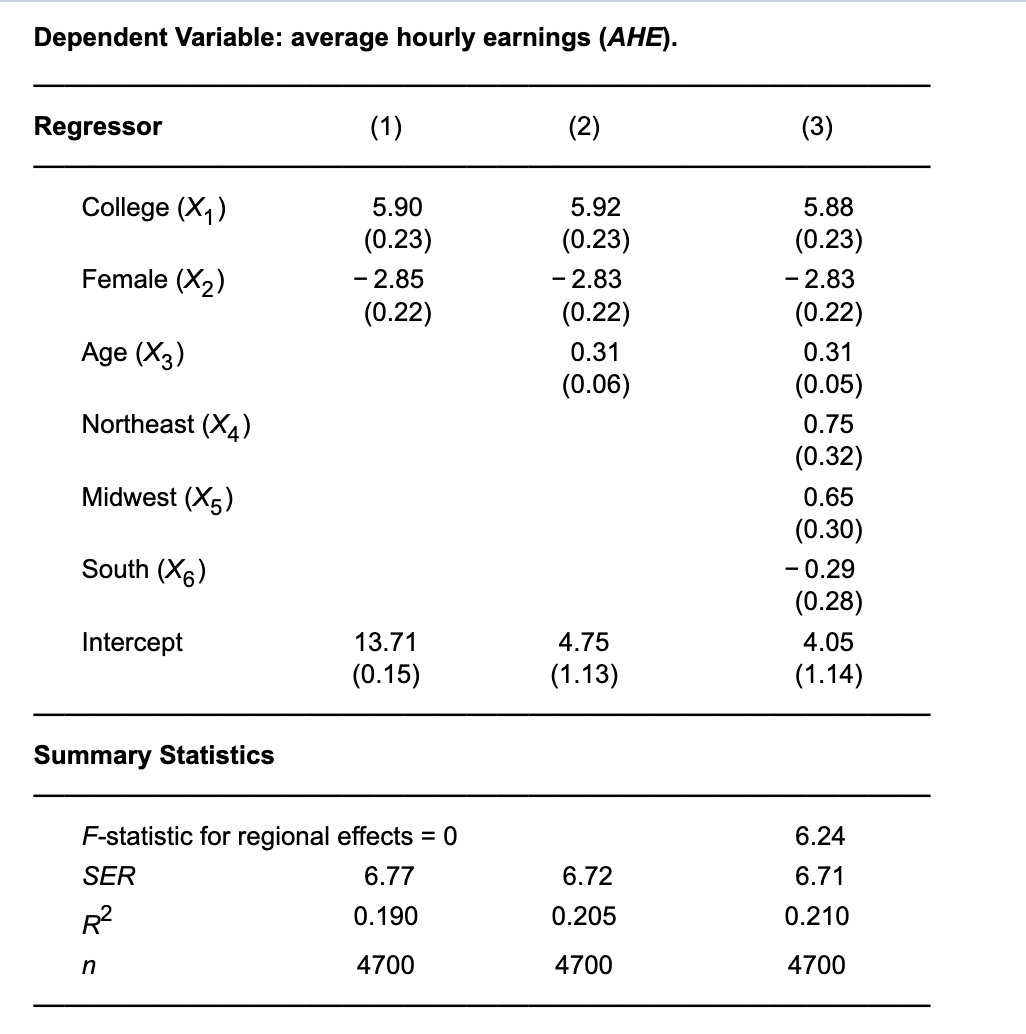
\includegraphics[scale=0.5]{materials/sw7-3.png}

\begin{longtable}[]{@{}ll@{}}
\toprule
Variable & Definition\tabularnewline
\midrule
\endhead
AHE & average hourly earnings (in 2005 dollars)\tabularnewline
College & 1 if college, 0 if high school\tabularnewline
Female & 1 if female, 0 if male\tabularnewline
Age & age (in years)\tabularnewline
Ntheast & 1 if Region = Northeast, 0 otherwise\tabularnewline
Midwest & 1 if Region = Midwest, 0 otherwise\tabularnewline
South & 1 if Region = South, 0 otherwise\tabularnewline
West & 1 if Region = West, 0 otherwise\tabularnewline
\bottomrule
\end{longtable}

\begin{enumerate}
\def\labelenumi{\arabic{enumi}.}
\setcounter{enumi}{4}
\tightlist
\item
  Consider the regression results below and do the following:

  \begin{enumerate}
  \def\labelenumii{\alph{enumii}.}
  \tightlist
  \item
    Construct the \(R^2\) for each of the regressions
    
        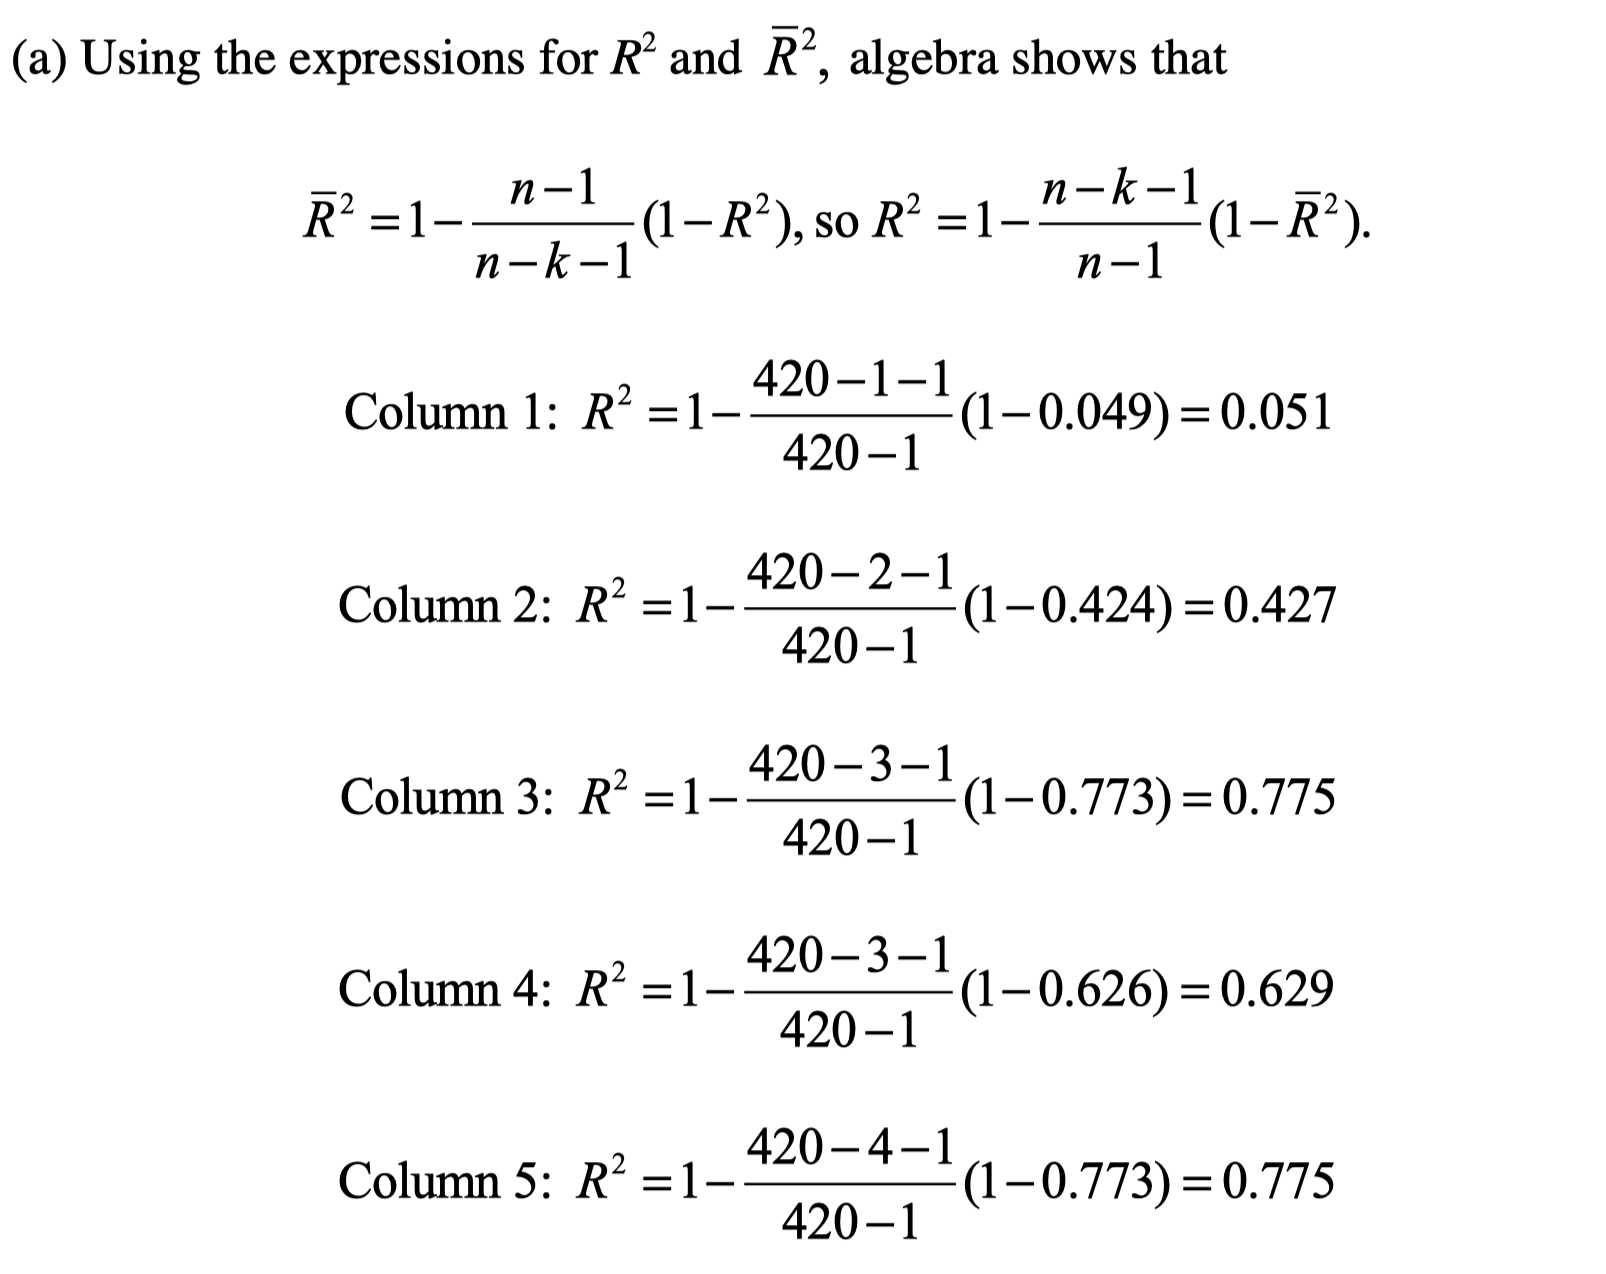
\includegraphics[scale=0.3]{solutions/ps4-q5a.png}

    
  \item
    Construct the homoskedasticity-only \(F\)-statistic for testing
    \(\beta_3 = \beta_4 = 0\) shown in column (5). Is the statistic
    significant at the 5\% level?
    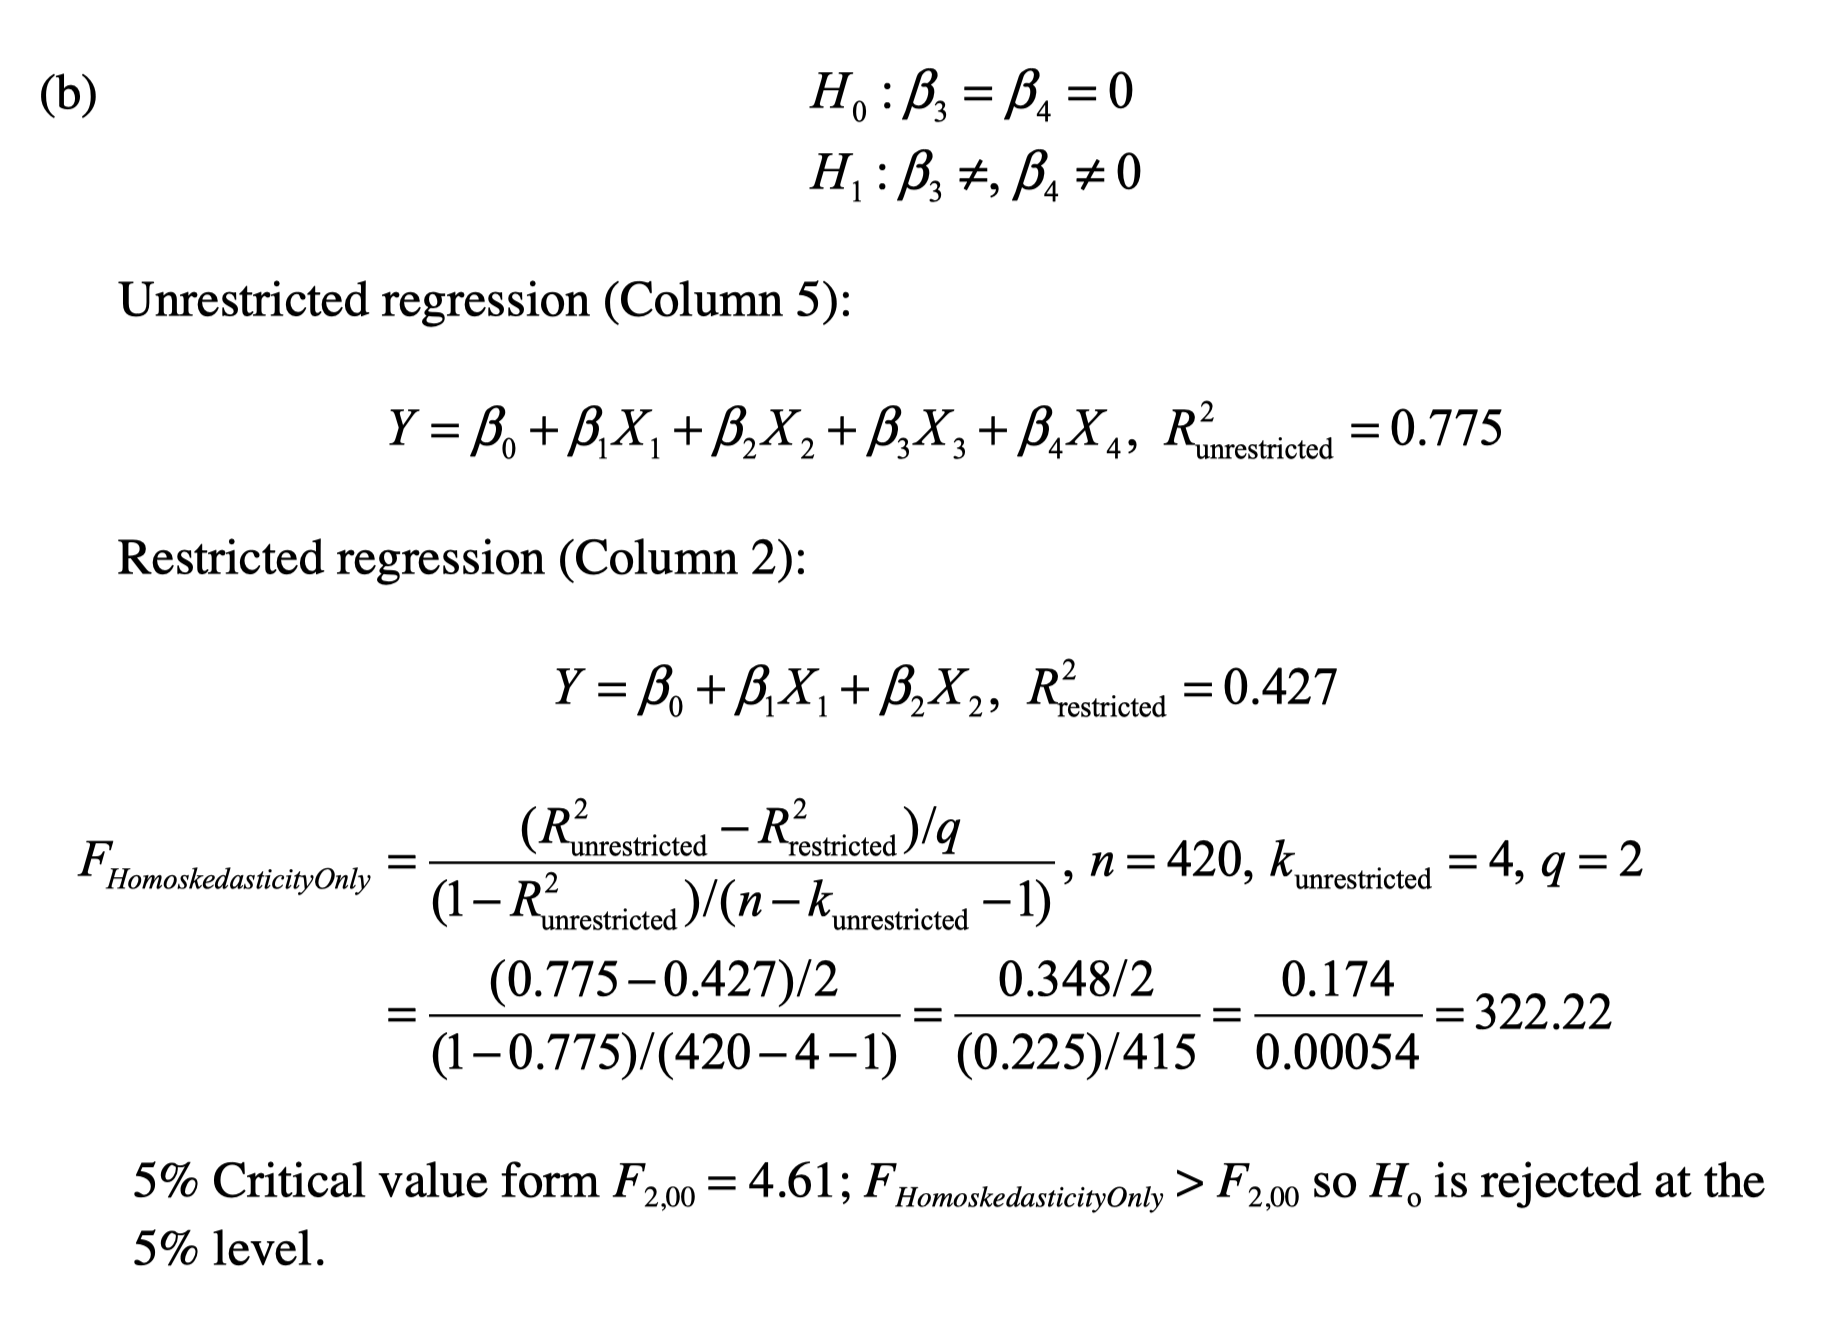
\includegraphics[scale=0.3]{solutions/ps4-q5b.png}
  \item
    Construct a 99\% confidence interval for \(\beta_1\) for the
    regression in column (5)
    
    {\color{red} 
    $-1.01 \pm 2.58*0.27$ 
    } 
    
  \end{enumerate}
\end{enumerate}

\centering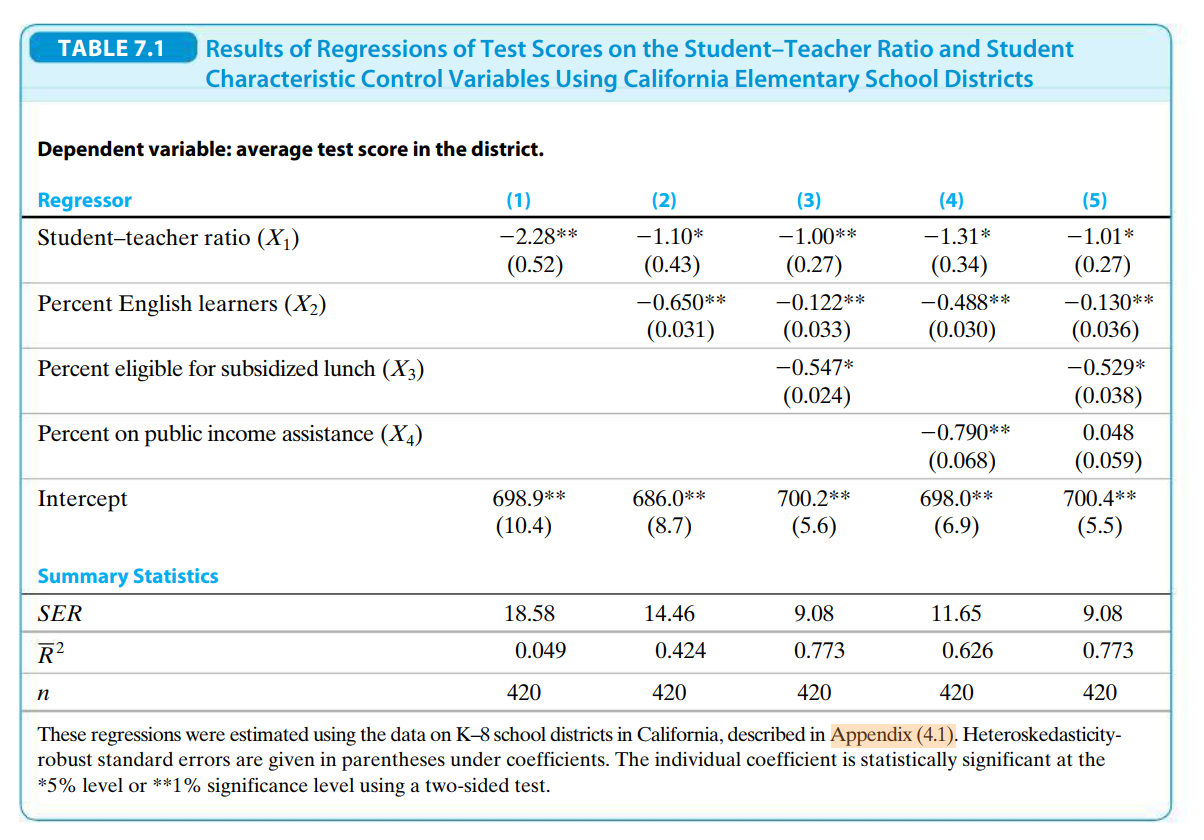
\includegraphics[scale=0.5]{materials/sw7-1.png}

\begin{enumerate}
\def\labelenumi{\arabic{enumi}.}
\setcounter{enumi}{5}
\tightlist
\item
  Download the dataset {growth.dta} from the website, which
  contains data on average growth rates from 1960 through 1995 for 65
  countries, along with variables that are potentially related to
  growth. You can download a detailed description of all variable names
  is available
  \href{https://www.princeton.edu/~mwatson/Stock-Watson_3u/Students/EE_Datasets/Growth_Description.pdf}{here}.
  For all questions, exclude Malta, which has an extremely high trade
  share. Estimate a regression of \texttt{growth} on
  \texttt{tradeshare}, \texttt{yearsschool}, \texttt{rev\_coups},
  \texttt{assassinations}, and \texttt{rgdp60}, with
  heteroskedasticity-robust standard errors.

  \begin{enumerate}
  \def\labelenumii{\alph{enumii}.}
  \tightlist
  \item
    What is the value of the coefficient on \texttt{rev\_coups}?
    Interpret the value of this coefficient. Is it large or small in a
    real-world sense?
    
  \item
    Use the regression to predict the average annual growth rate for a
    country has average values for all regressors.
  \item
    Construct a 90\% confidence interval for the coefficient on
    \texttt{tradeshare}. Is the coefficient statistically significant at
    the 10\% level? d.Test whether the political variables
    \texttt{rev\_coups} and \texttt{assassinations}, taken as a group,
    can be omitted from the regression. What is the p-value of the
    F-statistic?
  \end{enumerate}
\end{enumerate}

{\color{red} See do-file}
\end{document}
